\documentclass{beamer}
\usetheme{Warsaw}
\usepackage{wrapfig}
\title{Chatting with OTR over Tor with VPN}
\author{Gavin Bauer, Ryan McCarthy, Amruta Dubewar}
\date{\today}
\defbeamertemplate*{footline}{shadow theme}
{%
  \leavevmode%
  \hbox{\begin{beamercolorbox}[wd=.5\paperwidth,ht=2.5ex,dp=1.125ex,leftskip=.3cm plus1fil,rightskip=.3cm]{author in head/foot}%
    \usebeamerfont{author in head/foot}\insertframenumber\,/\,\inserttotalframenumber\hfill\insertshortauthor
  \end{beamercolorbox}%
  \begin{beamercolorbox}[wd=.5\paperwidth,ht=2.5ex,dp=1.125ex,leftskip=.3cm,rightskip=.3cm plus1fil]{title in head/foot}%
    \usebeamerfont{title in head/foot}\insertshorttitle%
  \end{beamercolorbox}}%
  \vskip0pt%
}

%2,4,5,6
\begin{document}
\begin{frame}
\maketitle
\end{frame}
\section{VPN}
\subsection{Setting up the VPN}
\begin{frame}
\frametitle{Install OpenVPN and Generate Static}
\begin{itemize}
\item OpenVPN installation command\\
\item \# sudo apt-get install openvpn\\
\item In the server's /etc/openvpn directory, run the following command to generate a static key:
\item	\# openvpn --genkey --secret static.key

\item Then file static.key get generated in /etc/openvpn folder. Copy this file static.key to the clients /etc/openvpn directory using a secure channel like scp or sftp.

\end{itemize}
\end{frame}
\subsection{Initiating connection}

\begin{frame}
\frametitle{Server Config}
\begin{columns}
    \begin{column}{0.48\textwidth}
	\begin{itemize}
	\item On Server Run below command:\\
	\item \# sudo openvpn {\color{red}{--proto tcp-server}} --remote \textless clientIP\textgreater  --dev tun0 --ifconfig 10.1.0.1 10.1.0.2 --verb 3 --comp-lzo yes --float --secret /etc/openvpn/static.key
        \end{itemize}
    \end{column}
    \begin{column}{.5\textwidth}
        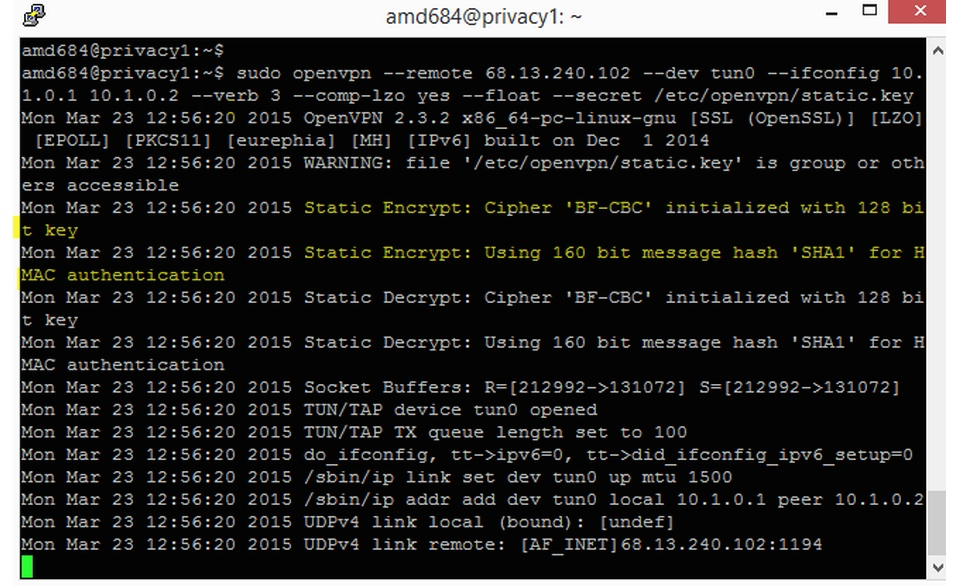
\includegraphics[width=.9\linewidth]{am1}
    \end{column}
\end{columns}
\end{frame}

\begin{frame}
\frametitle{Client Config}
\begin{columns}
    \begin{column}{0.48\textwidth}
        \begin{itemize}
	\item On Client Run below command:\\
	\item \# sudo openvpn {\color{red}{--proto tcp-client}} --remote \textless remoteIP\textgreater  --dev tun0 --ifconfig 10.1.0.2 10.1.0.1 --verb 3 --comp-lzo yes --secret /etc/openvpn/static.key
        \end{itemize}
    \end{column}
    \begin{column}{.5\textwidth}
        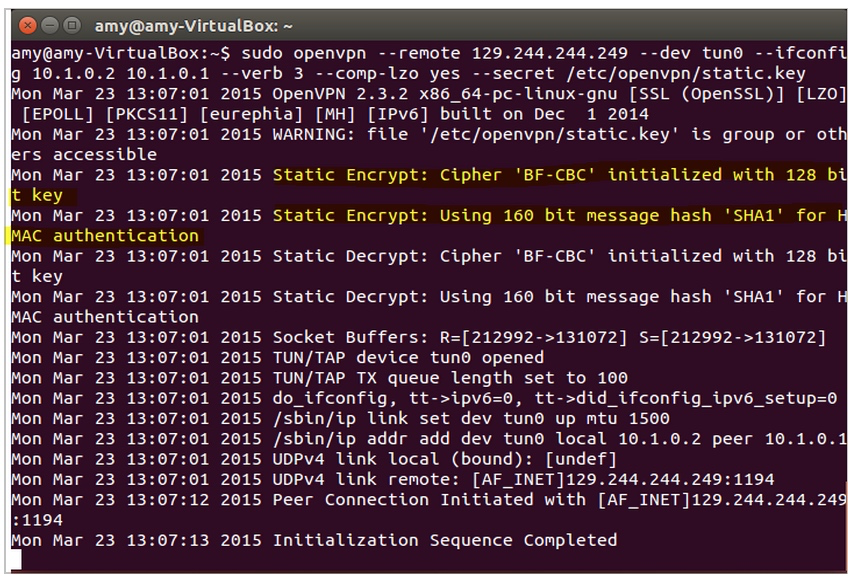
\includegraphics[width=.9\linewidth]{am2}
    \end{column}
\end{columns}
\end{frame}

\subsection{Verify Tunnel}
\begin{frame}
\frametitle{Verify Tunnel}
\begin{columns}
    \begin{column}{0.48\textwidth}
        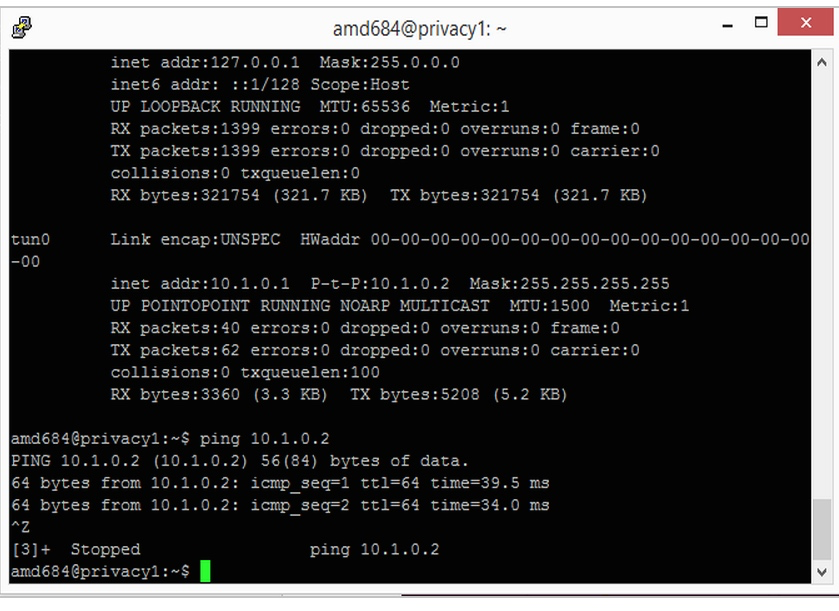
\includegraphics[width=.9\linewidth]{left}
    \end{column}
    \begin{column}{.5\textwidth}
        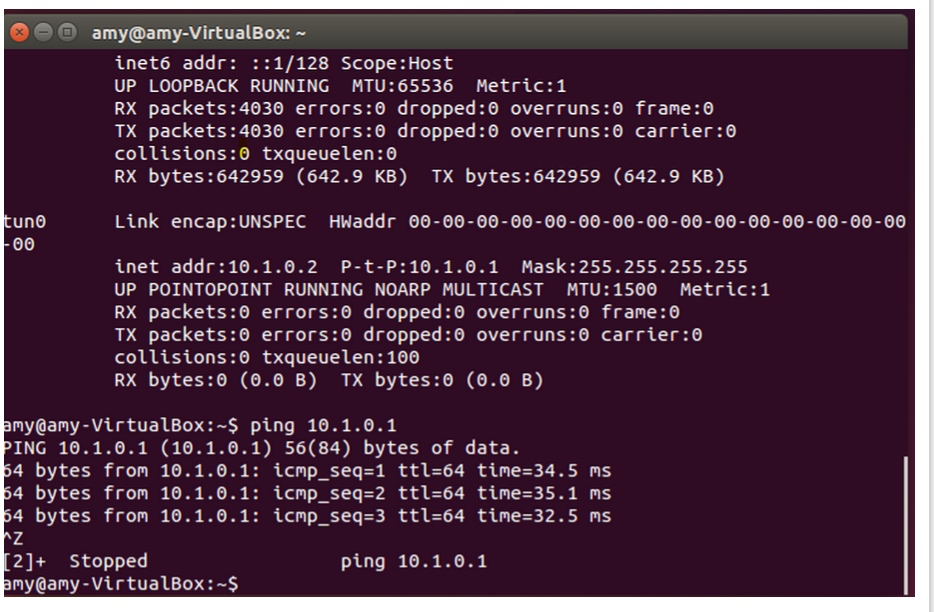
\includegraphics[width=.9\linewidth]{right}
    \end{column}
\end{columns}
\end{frame}


\section{VPN}
\subsection{Tor and the VPN}
\begin{frame}
\frametitle{Piping OpenVPN over Tor}
\begin{itemize}
\item To get OpenVPN to go over Tor OpenVPN must use TCP rather than UDP
\item Install torsocks
\item Run tor and then do torsocks plus the OpenVPN command
\end{itemize}
\end{frame}

\section{Tor}
\subsection{Installing Tor}
\begin{frame}
\frametitle{Installing The Onion Router}
\begin{itemize}
\item For Linux: Tor is just a simple apt-get away:\\
\pause
{\color{blue}{sudo apt-get install tor}}
\pause
\item For Mac: Homebrew or Ports should be installed first:\\
\pause{\color{blue}{brew install tor}} Or {\color{blue}{ports install tor}}
\pause
\item For Windows:
\pause
{\color{red}{You're on your own...}}

\end{itemize}
\end{frame}

\subsection{Chat Client Address Configuration}
\begin{frame}
\frametitle{Adium Configuration}
\begin{columns}
    \begin{column}{0.48\textwidth}
        \begin{itemize}
          \item Step one: Open Preferences
	 \item Step two: Click on the Options tab under General Settings
          \item Step three: Enter the hidden service url in the Connect Server box
        \end{itemize}
    \end{column}
    \begin{column}{.5\textwidth}
        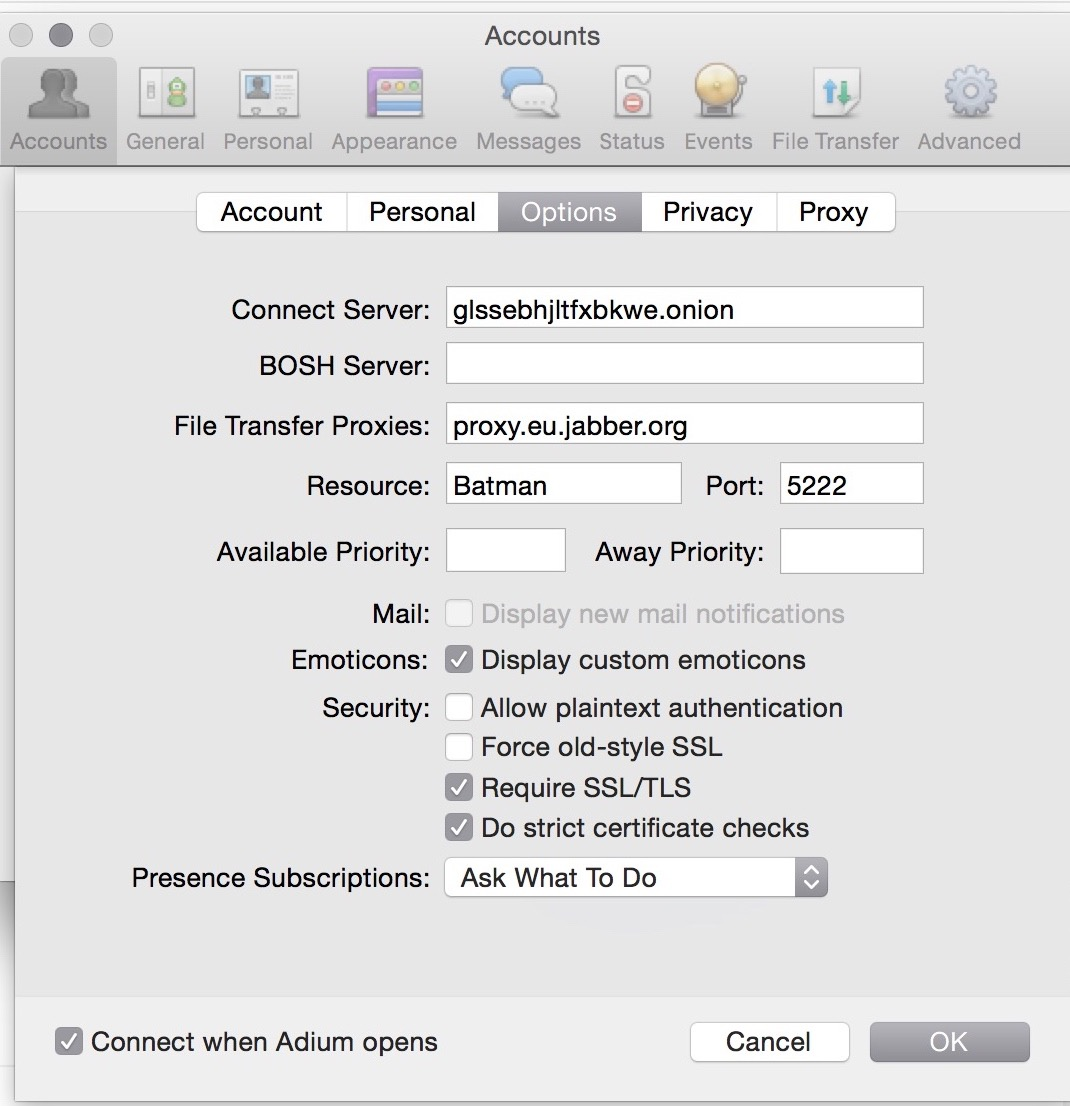
\includegraphics[width=.9\linewidth]{adium1}
    \end{column}
\end{columns}
\end{frame}

\subsection{Chat Client Proxy Configuration}
\begin{frame}
\frametitle{Adium Configuration}
\begin{columns}
    \begin{column}{0.48\textwidth}
        \begin{itemize}
          \item Step four: Click on the Proxy tab
	 \item Step five: Select Socks5 for the proxy
	 \item Step six: The address is localhost or 127.0.0.1
	 \item Step seven: The proxy port is 9050
        \end{itemize}
    \end{column}
    \begin{column}{.5\textwidth}
        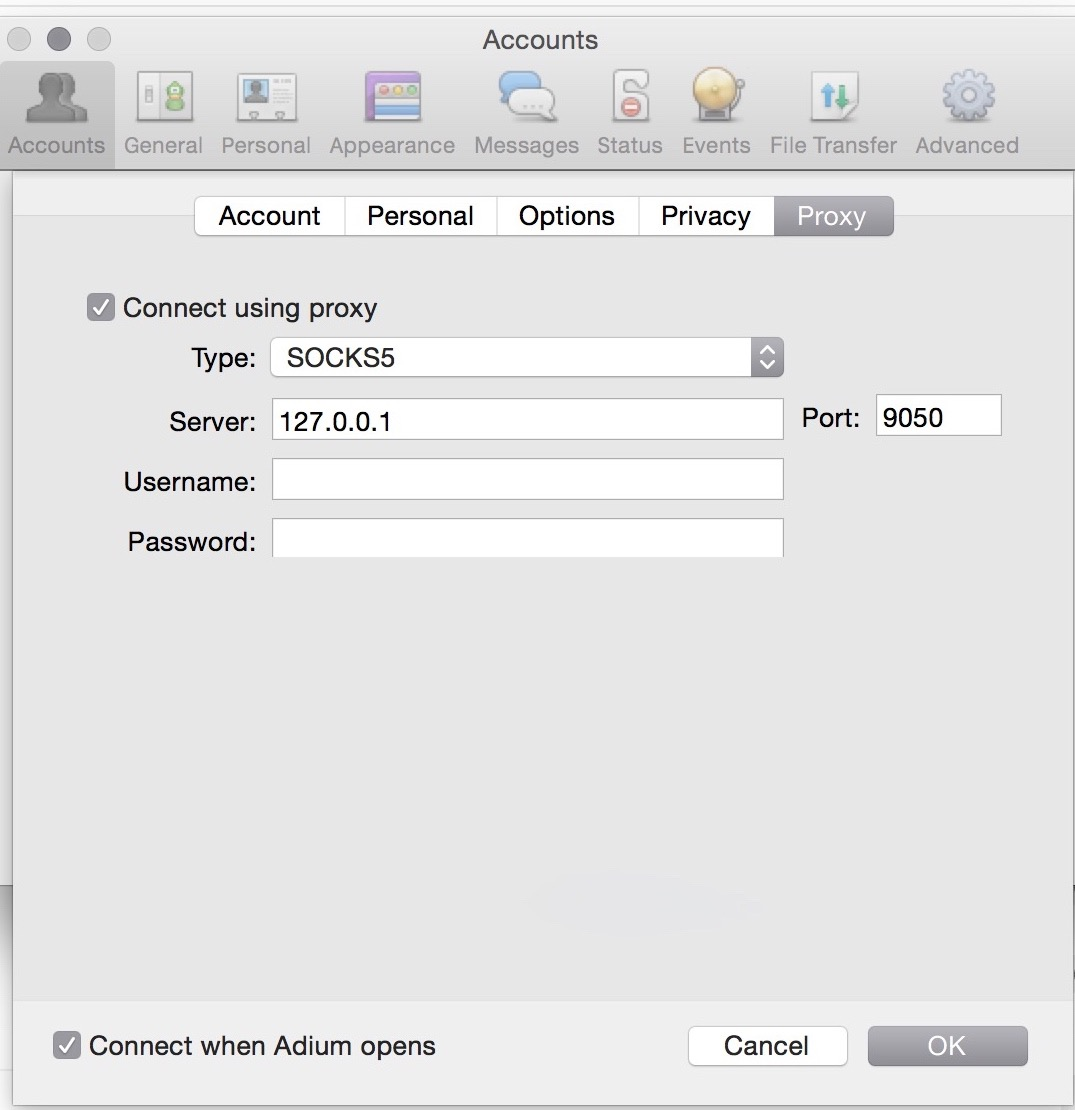
\includegraphics[width=.9\linewidth]{adium}
    \end{column}
\end{columns}
\end{frame}

\section{Pidgin}
\subsection{How Pdigin Integrates}
\begin{frame}
\frametitle{How Pidgin Integrates}
\begin{itemize}
\item Pidgin (any others) has built-in proxy utility
\item All traffic is piped through proxy
\item Then traffic is routed to .onion server
\item Then traffic is forwarded to XMPP server
\end{itemize}
\end{frame}
\subsection{Setting up Pidgin}
\begin{frame}
\frametitle{Setting up Pidgin}
\begin{columns}
    \begin{column}{0.48\textwidth}
        \begin{itemize}
          \item Modify your account
          \item Go to Advanced
        \end{itemize}
    \end{column}
    \begin{column}{.5\textwidth}
        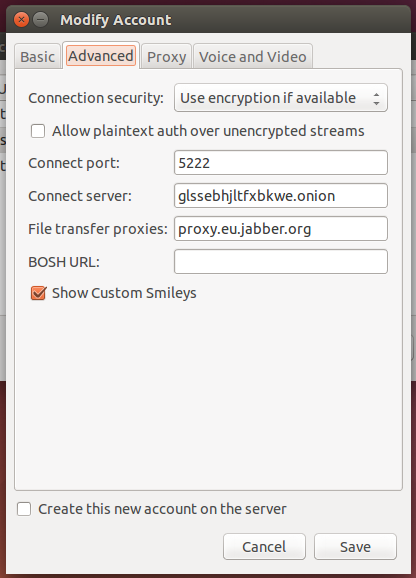
\includegraphics[width=.9\linewidth]{pidgin_advanced}
    \end{column}
\end{columns}
\end{frame}
\begin{frame}
\frametitle{Setting up Pidgin}
%\item Go to Advanced\\
\begin{columns}
    \begin{column}{0.48\textwidth}
        \begin{itemize}
          \item Go to Proxy
        \end{itemize}
    \end{column}
    \begin{column}{.5\textwidth}
        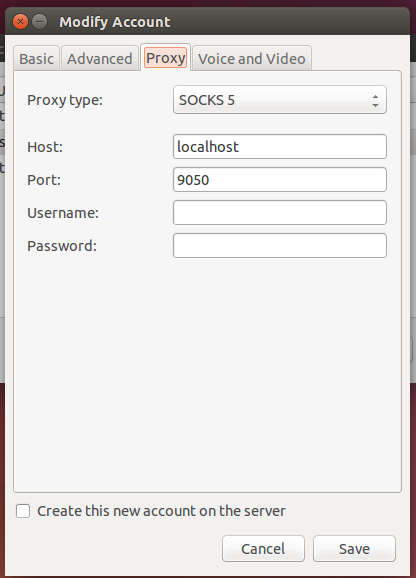
\includegraphics[width=.9\linewidth]{pidgin_proxy}
    \end{column}
\end{columns}
\end{frame}
\subsection{Verifying pdigin}
\begin{frame}
\frametitle{Verifying Pidgin}
\begin{columns}
    \begin{column}{0.48\textwidth}
        \begin{itemize}
          \item Login to the privacy box
          \item Attempt to OTR chat with someone
        \end{itemize}
    \end{column}
    \begin{column}{.5\textwidth}
        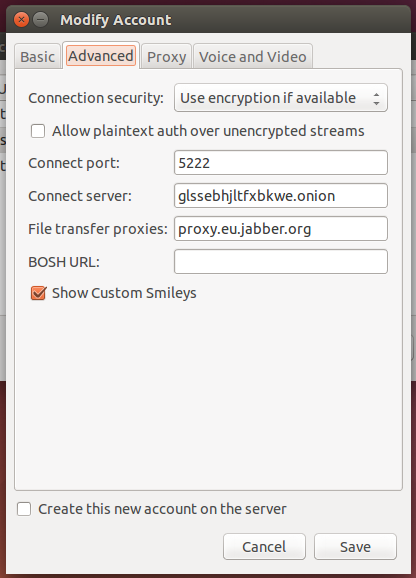
\includegraphics[width=.9\linewidth]{pidgin_advanced}
    \end{column}
\end{columns}
\end{frame}
\section{Summery}
\begin{frame}
\frametitle{Summery}
\begin{center}
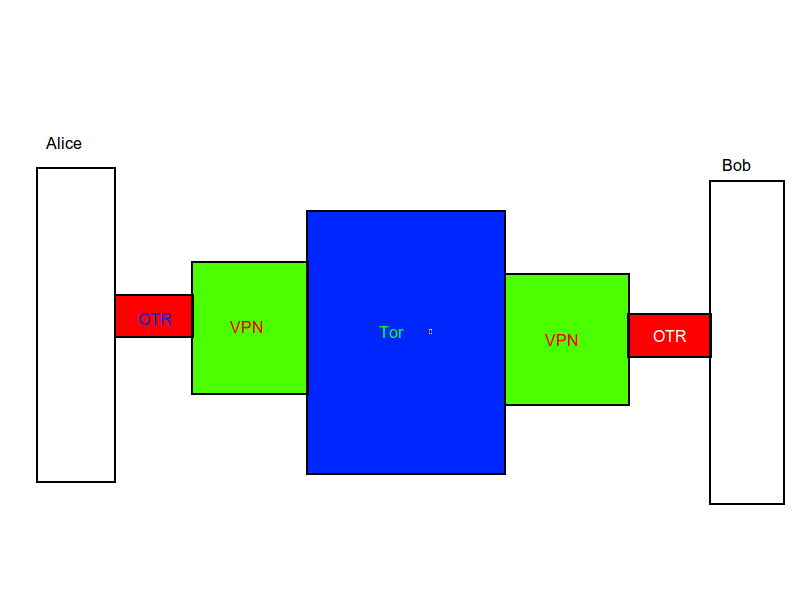
\includegraphics[width=1\linewidth]{overview}
\end{center}
\end{frame}
\section{Fin}
\end{document}
